\begin{refsection}
\chapter{Feature Selection and Model Regularization}

\begin{summary}
The data may contain features that are either redundant or irrelevant, and their removal may have no or only small effect on model accuracy. The reduction of feature space may also help us avoid overfitting. By selecting the most informative features, we may reduce running times and computational complexity and increase the interpretability of results due to the inference of simpler models. Three main approaches to feature selection use filter, wrapper, and embedded methods. In the filter approach, we select the most informative features before modeling. Wrapper methods select features according to the observed performance of inferred models and treat the modeling technique as a black box. With embedded methods, we refer to modeling techniques, which include feature selection within a model inference procedure. In this chapter, we will dive into filter and wrapper approaches, and for embedded methods focus on model regularization.
\end{summary}

\section{Relation to Dimensionality Reduction}

Dimensionality reduction is an essential part of quantitative data analysis whose aim is to reduce the dimensions of the data considered in the inference of the model. A positive effect of dimensionality reduction is a decreased model complexity and shortened inference time. Another potential benefit is increased interpretability due to the inference of simpler models. The central premise of dimensionality reduction is that this procedure will have little or no effect on the accuracy of the model. 

Dimensionality reduction is effective if the input data includes redundant or irrelevant features, or if we can use new features to replace a subset of original features so that to encapsulates all their information. The three most common families of approaches for dimensionality reduction are:
\begin{itemize}
\item {\em Feature transformation} that embeds the data into a lower-dimensional space, replacing original features with a new set that retains as much of information as possible. Approaches of this kind include principal component analysis and deep autoencoders, some of which we will cover in later chapters.
\item {\em Feature selection}, also known as feature subset selection, variable selection, or attribute selection. This approach removes the dimensions (\eg columns) from the input data and results in a reduced data set for model inference.
\item {\em Regularization}, where we are constraining the solution space while doing optimization. Here, we add adding the regularisation terms to which an optimization algorithm must adhere to when minimizing the loss function, apart from having to minimize the error between the true $y$ and the predicted $\hat{y}$. In lasso regularization, for instance, optimization is instructed to find model parameters so that their absulute sum is minimized. This type of regularization may lead to some of the parameters be equal to zero, effectively imposing zero weight to corresponding features, essentially canceling them out from the model. Hence, regularization can be also regarded as a feature selection, where the selection procedure is embedded within an inference method.
\end{itemize}

\ifguide{
The students should already be familiar with the terms feature transformation and feature selection and they have applied feature transformations methods (PCA) and basic 'manual' feature selection. See \url{https://fri-datascience.github.io/course_ids/handbook/multivariate-data-chapter.html}.
}

\section{Feature Selection}

\ifguide{
ESL and Murphy books have very little on this. A good reference for students is ISL (6.1.2), which covers forward and backward and mentions hybrid. For the rest, rely on these notes or possibly find other references.
}

Feature selection is an optimization problem. The search space is the set of all possible subsets of features, that is, the power set, with $2^n$ possible solutions. We are trying to find the best solution under some utility and constraints. An example of utility could be the accuracy of the model when inferred from the reduced feature set, and a constraint may be expressed through a maximal number of features. Viewing feature selection as an optimization problem leads to the following properties of the procedure:
\begin{itemize}
\item Because we have a discrete search space, we can, in general, not find the optimal solution, unless we perform a global search and evaluate all $2^n$ solutions.
\item Unless the number of original features $n$ is very small, examining all $2^n$ solutions is infeasible.
\item In practice, the best we can do is to use heuristic search methods with a good inductive bias. This approach tends to work well because we can impose assumptions that are more likely to hold on the data we encounter.
\item Any search method that operates on discrete search spaces can also be applied to feature selection.
\end{itemize}

\subsection*{Filter Methods}

Filter methods~\citep{Guyon2003} perform feature selection before the inference of the model. They rely on a feature scoring function that assigns the score to a feature according to how useful the feature could be in the model. Notice that the scoring is performed before and independently of the model. Features are scored and then ranked, and usually, a top $k$ features are selected, where $k$ is a user-defined parameter of the procedure. Alternatively, feature scores could be compared to their null-distribution that, in practice, could be obtained through feature scoring on a randomly permuted data set. In such cases, $k$ is replaced with user-defined probability $p$ that a particular (or higher) feature score could be obtained and randomly-permuted data.

Scoring functions depend on the type of machine learning problem and type of the scored feature. For instance, for unsupervised learning, we may disregard features with near-constant values by selecting features with the highest deviance, that is, with the highest ratio between variance and the mean. Scoring functions for classification or regression most often consider the correlation between a predictor and the dependent variable. One of the most popular empirical estimates is the mutual information between the $i$-th predictor and the target $y$ ~\citep{Guyon2003} :
$$
I(i)=\int_{x_i}\int_y p(x_i,y)\log{p(x_i,y)\over p(x_i)p(y)}dx dy,
$$
where $p(x_i)$ and $p(y)$ are the probability densities of predictor $x_i$ and dependent variable $y$, and $p(x_i,y)$ is their joint density. These densities are all unknown and are hard to estimate from the data. The easiest of all is the case of nominal variables, where integral becomes a sum and where probabilities are then estimated from frequency counts:
$$
I(i) = \sum_{x_i}\sum_{y} P(X=x_i, Y=y)\log {P(X=x_i,Y=y)\over P(X=x_i) P(Y=y)}.
$$

Notice that mutual information and all similar feature scoring techniques are univariate and assess the information held by the feature in the absence of the context of other features. The scoring function of this type would undervalue features that are in some interactions with other features and only combined with these provide information about the class. A typical example of such a combination is an exclusive disjunction, where participating features may provide no information about the class on their own, yet are information-rich when they are considered together with complementing argument. A field that studies the discovery and ranking of such features is called feature interaction analysis~\citep{Jakulin2005,Anastassiou2007}. The approaches cited here rely on an exhaustive search for feature interactions, which are prohibitive in complexity even for reasonably-sized data sets. A bigger problem, though, is that estimates of feature interactions may report about highly interactive features simply by chance and due to extremely high number of feature combinations explored.

Interestingly, however, note that there are feature score estimators that take into consideration the contexts and are sensitive to feature interactions. The most prominent of these is Relief, an algorithm originally developed by~\citet{Kira1992}. The algorithm assumes that each feature in the data set has been scaled to the interval $[0,1]$. Let $\vect{w}$ be a feature weight vector initialized to $\vect{0}$. The algorithm randomly draws a data instance $\vect{x}_i$ and updates the weight vector, such that:
$$
\vect{w}\gets\vect{w}-\left(x_i - {\rm nearHit}(x_i)\right)^2 + \left(x_i - {\rm nearMiss}(x_i)\right)^2
$$
where ${\rm nearHit}(x_i)$ is the closest same-class data instance to $x_i$, and ${\rm nearMiss}(x_i)$ is the closest different-class data instance to $x_i$. Notice that the weight of any given feature decreases if it differs from that feature in nearby instances of the same class more than nearby instances of the other class, and increases in the reverse case. In a local neighborhood, the best features should distinguish between instances of the different class and should be similar across instances of the same class. The score $\vect{w}$ is updated for $m$ random draws, and the features with the highest scores are those that should be selected. 

Several extensions and improvements of Relief were proposed by~\citep{Kononenko1997}. On the surface, Relief looks like a perfect feature scoring algorithm that can indeed cope with any hidden feature interactions. However, it relies on finding similar data instances and thus suffers from the same problem as any nearest neighbors approach. In other words, Relief would start failing in data sets with a higher number of features, which is precisely where feature interaction discovery would be of the highest value.

\subsection*{Wrapper Methods}

Wrapper methods score feature sets according to estimated accuracy or utility of the algorithm used for learning. The most common search approach are forward/backward stepwise selection~\citep{Guyon2003}. Forward selection is an iterative procedure that starts with an empty set of features and adds one feature at a time, where the benefit of adding a feature is observed in raised accuracy of the inferred model when that feature is added to the feature set. Backward selection starts with a full set of features, and then eliminates one feature at the time, each time selecting feature with the smallest impact on the accuracy of the model. Notice, of course, that backward selection can actually increase the accuracy of the model, as we expect that there is an optimal feature subset with corresponding highest accuracy.

Forward and backward stepwise selection do not necessary yield the same feature sets. Notice that in the presence of strong feature interactions (\eg consider exclusive disjunction) forward selection would miss including features that interact, while backward selection may leave interactive features in the selected set, provided that the underlying machine learning algorithm can detect and use the interactions.

There are other, more elaborate discrete space search procedures that could be used in combination of the wrapper approaches. Consider, for instance, local search algorithms, simulated annealing, or genetic algorithms.

\subsection*{Embedded Methods}

Embedded methods refer to feature selection techniques that are part of the learning algorithm itself. A typical example of such a method are classification trees, where the inferred model often includes only a subset of most informative features. Perhaps more elaborate technique in this respect are random forests, where the set of used features may be larger than those from a single tree and where out-of-bag examples can be used for feature scoring and hence ranking. 

Below, we will consider a special approach to embedded feature selection that is based on regularization, a constrained optimization that jointly considers accuracy of the inferred model and the magnitude of model parameters and with it the coplexity of the model.

\subsection*{A Rough Summary on Feature Selection Techniques}

Of the three approaches to feature selection stated above, wrapper methods are the most general and may yield the best results, but are computationally intensive and often infeasible even with simple brute force forward or backward search. This is especially the case with data domains which include tens or houndreeds of thousands of features that are common in areas like genomics, text, sound and image mining. Filter methods typically work one-feature-at-a-time and are faster, but they might provide suboptimal results, because the selection is decoupled from actual learning. Embedded methods are kind of the best of both worlds, but they require adaptation of the algorithm that implements them.

We already mentioned other approaches to dimensionality reduction that, instead of feature selection, rely on inference of new set of (latent) features. Examples of such feature transformation techniques include matrix factorization, principal component analysis, and deep autoencoders. In comparison with these techniques, please note that:
\begin{itemize}
\item feature selection has an advantage over feature transformation as it keeps the original features, which helps with interpretability,
\item feature selection is related to explanation/interpretability also through methods that assess variable importance, that is, provides a ranked set of features which can be scrutinized by the domain experts,
\item as computational power grows and data sets get larger, filter methods are used less and less and give way to models whose inference relies on optimization and gradient-based search of parameter space.
\end{itemize}


\section{Regularization}

\ifguide{
The students should already be familiar with key concepts from statistics (maximum likelihood estimation - MLE, parametric models, linear regression - including the relationship between least squares and MLE, Bayesian statistics) and optimization (convex optimization Lagrange multipliers, KKT, etc.). 
}


\ifguide{
ESL chapter 3.4 (Shrinkage methods), without Least angle regression, covers most of the material here. But it is important that all material in these notes is covered in the lecture and 3.4 is used as a complement - we can cover things more precisely, because of what our students know from previous courses. Murphy covers bits and pieces of L1 in 13.3 (up to and including 13.3.4; the rest are details and optimization algorithms). Murphy 7.5 on Ridge regression is also worth a read, but it gets very specific after first two subsections.

Additional readings:
\begin{itemize}
\item Tibshirani, R. (1996). Regression shrinkage and selection via the lasso. Journal of the Royal Statistical Society: Series B (Methodological), 58(1), 267-288. (read the first two sections for a basic understanding of Lasso and intuition behind how it compares with L2)
\item Park, T., \& Casella, G. (2008). The Bayesian lasso. Journal of the American Statistical Association, 103(482), 681-686. (to get an understanding of the Bayesian view on Lasso and approach with hyperparameter estimation, read the first three sections; before they can fully understand the inference, we need to cover Gibbs sampling in Math 2)
\end{itemize}
}

%TODO and quickly restate that the MLE estimator is the same as the least squares estimator.

Let us start with considering linear regression, where $\y_i = \b^\tr \x_i + \epsilon_i$ and where we assume that the error term is distributed normally, so that $\epsilon_i \sim_\text{iid} N(0, \sigma^2)$. The data, conveniently, includes a constant column, such that $x_0=1$, consequently using $\b_0$ as an intercept, a constant term in linear combination. Linear regression aims to find $\b^*$ that minimizes residual sum of squares,
\begin{align*}
{\rm RSS}(\b) & = \sum_{i=1}^n (\y_i-f(\x_i))^2 \\
& = \sum_{i=1}^n (\y_i - \b^T\x_i)^2 
\end{align*}
so that
$$\b_{\rm OLS} = \argmin_{\b} \sum_{i=1}^n (\y_i - \b^T\x_i)^2.$$
Notice that this criteria function actually stems from the maximum likelihood estimation, where parameters $\b$ are estimated by maximizing a likelihood function, so that under the assumed statistical model the observed data is most probable.

Linear regression also has a closed form solution~\cite{ESL}. Let $\X$ denote $n\times (1+p)$ matrix with $n$ training data instances described with $p$ features. The first column of the matrix is a unit vector. Residual sum of squares can then be expressed as:
$$
{\rm RSS}(\b) = (\y-\X\b)^\tr (\y-\X\b)
$$
Differentiating with respect to $\b$ we obtain 
\begin{eqnarray*}
\frac{\partial{\rm RSS}}{\partial \b} & = & -2\X^\tr (\y - \X\b) \\
\frac{\partial^2{\rm RSS}}{\partial^2\b} & = & -2\X^\tr\X
\end{eqnarray*}
Setting the first derivative to zero and assuming that $\X$ is nonsingular and hence $\X^\tr\X$ is positive definite, we obtain
\begin{eqnarray*}
\X^\tr (\y - \X\b_{\rm OLS}) & = & 0 \\
\b_{\rm OLS} & = & (\X^\tr\X)^{-1}\X^\tr\y
\end{eqnarray*}

The main problem that we will address with regularization are cases with few observations in the data set that are described with comparably many features. In other words, cases where the training data matrix $\X$ has relatively few rows compared with columns. Here, we are likely to overfit the data, that is, develop a complex model that includes many features and fits training data well but misperforms in prediction on new data. In fact, if we have more columns than rows, we will have colinearity, so $\X^\tr\X$ will not be invertible and if we want to solve it by minimizing the sum of squares, we will have an infinite number of equivalent solutions.

We will look at regularization from a few different perspectives. The first and the most commonly used one is addressing the overfit by penalizing deviations of model coefficients from zero. For linear regression, if the value of a coefficient is 0, we regard that the corresponding feature is not used in the model. A common approach to supress the magnitude of model coefficients is to use a quadratic penalty term, leading to the modified optimization problem:
$$
\b_{L2} = \argmin_{\b} \left(\sum_{i=1}^n (\y_i - \b^\tr\x_i )^2 + \lambda \sum_{i=1}^k \b_i^2\right),
$$
where $\lambda \geq 0$ is the regularization parameter or regularization weight. Notice that $\lambda$ is an additional parameter of the optimizatio problem whose value must either be set manually or determined through some optimization procedure that can involve estimation of accuracy of resulting model by cross-validation or using a validation data set. There are two extreme regularization cases: if $\lambda = 0$, we get non-regularized regression; if $\lambda=\infty$, the regularization penalty is so high that the optimal solution is to select $\b_i = 0$ for all $i\geq 1$. Note that the intercept, $\b_0$, is not regularized and in this case becomes equal to the mean value of the outcome variable. The optimal value of $\lambda$ lies somewhere between these two extremes, and penalizes the coefficients just enough to prevent overfitting, but not too much to interfere with the learning, that is, not obfuscating the likelihood term.

The quadratic (L2 norm) penalty is not the only one we can use. We will later discuss the other commonly used penalty, the absolute or L1 norm penalty. And we can here note that another, potentially useful penalty uses the L0 norm (counting), which penalizes for the number of features selected, that is, the number of nonzero $\b_i$. But first we will explore how L2 penalty term transforms the initial optimization problem of finding the maximum of the likelihood.

\subsection*{Closed-Form Solution for L2 Regularization}

Similar to how we derived the above closed-form solution to the least squares problem we can also derive a closed-form solution to the penalized regression. We want to minimize $\left(\sum_{i=1}^n (\b^T\x_i - \y_i)^2 + \lambda \sum_{i=1}^k \b_i^2\right)$ or, in matrix shorthand $\lVert \X\b - \y \rVert^2_2 + \lambda\lVert \b \rVert^2_2$. Again, we find the extreme the usual way by differentiating and checking where the gradient is 0:

$$\frac{d}{d\b} \left(\lVert \X\b - \y \rVert^2_2 + \lambda\lVert \b \rVert^2_2\right) = 2(\X\b - \y)^\tr \X + 2\lambda\b = 2\b^\tr\X^\tr\X - 2\y^\tr\X + 2\lambda\b^\tr$$

Note that if we differentiate again, we get $2\X^\tr\X + 2\lambda \I$. This is always positive definite for $\lambda > 0$, so we have a minimum. This is in contrast with non-penalized regression, where we rely on the additional assumption that $\X$ has full rank, making $2\X^\tr\X$ positive definite by itself.

Finally, the extreme is where the gradient is zero, so that $2\X^\tr\X\b_{L2} - 2\X^\tr\y + 2\lambda\b_{L2} = (2\X^\tr\X + 2\lambda \I)\b_{L2} - 2\X^\tr\y = 0$ or $ (\X^\tr\X + \lambda \I)\b_{L2} = \X^\tr\y $, which leads to
$$\b_{L2} = (\X^\tr\X + \lambda \I)^{-1}\X^\tr\y$$.
%
Note that the term is invertible for the reasons discussed above. In essence, we make $\X^\tr\X$ invertible by adding at least a tiny number to its diagonal elements, making the resulting matrix invertible even if it was not invertible by itself. Besides constraining the solution space, L2 regularization solves the problem of non-invertibility that we can encounter when using plain linear regression.

\subsection*{Equivalence of Penalized and Constrained Forms}

\ifguide{
ESL states this equivalence of constrained and penalized formulations but provides no background. We can do better and tie it to what students already know from math.
}

L2 regularization, as stated above, can be viewed as penalized optimization, where we deal with the objective and a penalty:

$$\text{minimize}_{\b} \left\{ \lVert \b^\tr\x_i - \y_i \rVert^2_2 + \lambda\lVert \b \rVert^2_2\right\}.$$
%
This optimization problem can be formulated as an alternative way that provides additional insight into what regularization does geometrically:

$$\text{minimize}_{\b} \left\{ \lVert \b^\tr\x_i - \y_i \rVert^2_2\right\}, \text{subject to }  \lVert \b \rVert^2_2 \leq c, $$
%
where $c \geq 0$ is some constant. Now we show that these two are indeed equivalent. We will use $\b_P$ to denote the solution to the penalized form and $\b_C$ the solution of the constrained form. First, we show that for any $\X$, $\y$, and every $c$ there exists a constant $\lambda$ that does not depend on $\X$ and $\y$ such that the solutions of the two problems are the same, that is, $\b_C = \b_P$. In other words, we will show that every constraint formulation of the problem has an equivalent penalized formulation.

We already know the solution to the penalized formulation (we derived it above):

$$\b_{P} = (\X^\tr\X + \lambda \I)^{-1}\X^\tr\y$$

Now we write the Lagrangian of the constrained formulation:

$$L(\b, \mu) =  \lVert \b^\tr\x_i - \y_i \rVert^2_2 + \mu (\lVert \b \rVert^2_2 - c)$$

According to Karush–Kuhn–Tucker (KKT), we have the following conditions to guarantee an optimal solution, which are in this case sufficient, because we have a convex problem and continuously differentiable constraints:
\begin{eqnarray}
\frac{d}{d\b} L(\b, \mu) & = & 0 \\
\mu & \geq & 0 \\
\mu (\lVert \b \rVert^2_2 - c) & = & 0
\end{eqnarray}
%
Observe that, for the first of the above conditions, the left hand side is the same as the gradient of the penalized form, just using $\mu$ instead of $\lambda$.

Now assume that $\b_P$ solves the penalized formulation for a given $\lambda$. Setting $\mu = \lambda$, $\b = \b_P$, and $c = \lVert \b_P \rVert^2_2$  satisfies all three KKT conditions, so there exists for every $\lambda$ a $c$ such that the solutions to the two problems are the same. Conversely, if $\b_C, \mu$ solves the constrained formulation for a given $c$, then $\b_C$ solves the penalized formulation at $\lambda = \mu$. So, there exists for every $c$ a $\lambda$ such that the solutions to the two problems are the same. Thus the formulations are equivalent.

In essence, we have shown that penalizing the solution with the quadratic norm is equivalent to putting a hypersphere constraint on the solution. This equivalence of constrained and penalized forms applies in general to $p$-norms~\citep{ESL}.

\subsection*{L1 regularization}

The optimization problem of L1 regularization, also known as Lasso regression, is:

$$\b_{L1} = \argmin_{\b} \left(\sum_{i=1}^n (\b^\tr\x_i - \y_i)^2 + \lambda \sum_{i=1}^k |\b_i|\right)$$
%
or, in vector notation: 
%
$$\b_{L1} = \argmin_{\b} \left( \lVert \b^\tr\x_i - \y_i \rVert^2_2 + \lambda\lVert \b \rVert_1\right).$$

With the result from the previous section on comparison of constrained and penalized formulation it is not too big a cheat if we immediately say that L1 is equivalent to a 'diamond' constraint, although the proof is not so obvious. This also allows for the geometric discussion of why Lasso regression tends to set coefficients to zero, while L2 regularization usually infers small but non-zero values of coefficients.

\begin{figure}
\centering{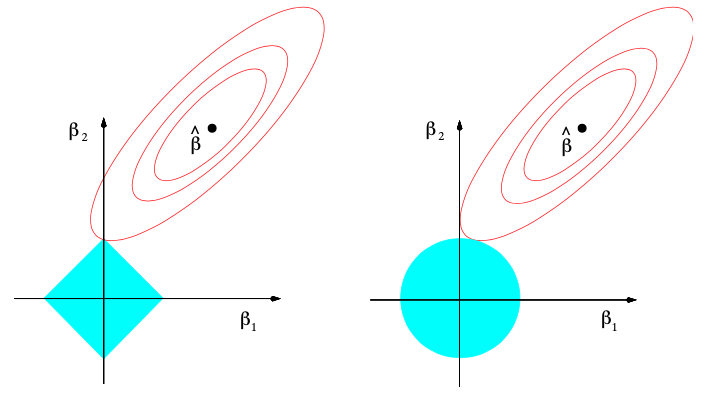
\includegraphics[width=0.7\linewidth]{figures/fss-l1-vs-l2.png}}
\caption{Geometric presentation of the optimization problem for the lasso (L1, left) and ridge (L2, right) regression. Shown are conturs of the penalty (least squares error), and the constrain regions $|\beta_1|+|\beta_2|\leq c$ and $\beta_1^2+\beta_2^2\leq t^2$. The sharp corners of the constraint region of the lasso yield sparse solutions. In high dimensions, sparsity arises from corners and edges of the lasso's constraint region (from~\cite{Tibshirani2014}).}
\end{figure}

\ifguide{
ESL has a good discussion of this geometric intuition and also of other norms. NOTE: Maybe go with $Lp$ norm directly ( $\lVert \b \rVert_p$) and introduce L1 as an important special case because of its feature subset selection properties.
}

\subsection*{Bayesian Interpretation of Regularization}

Regularization is sometimes referred to as \emph{a bet on sparsity}. That is, we are making an apriori assumption that not all (or even not most) of the input variables are relevant predictors. As soon as we introduce prior information it should not come as a great surprise that regularization has a very elegant Bayesian interpretation.

To see this, we go back to the optimization goal of ordinary least squares regression from the beginning of the chapter:

$$\b_{OLS} = \argmin_{\b} \sum_{i=1}^n (\b^\tr\x_i - \y_i)^2,$$
%
and recalling that this minimization is equivalent to maximizing the normal (Gaussian) likelihood assumed by the linear regression model,
%
$$L(\b;...) = \prod_{i=1}^n \frac{1}{\sqrt{2\pi\sigma^2}}\exp(-\frac{(\b^\tr\x_i - \y_i)^2}{2\sigma^2})$$
Indeed, maximizing the log-likelihood, we obtain
 
$$\ell(\b;...) = \sum_{i=1}^n \log\frac{1}{\sqrt{2\pi\sigma^2}} - \frac{1}{2\sigma^2}\sum_{i=1}^n(\b^\tr\x_i - \y_i)^2$$
%
Note that the maximum w.r.t. the $\b$ does not depend on $\sigma^2$, only on mimimizing the sum of squares.

With what do we have to multiply the likelihood to produce the extra term $-\lambda \sum_{i=1}^k \b_i^2$ in the log-likelihood and therefore get the negative of this term which appears in the minimization problem of L2 regression? 

The answer should be obvious: $\prod_{i=1}^k\exp(-\frac{\b_i^2}{1 / \lambda})$. In terms of $\b_i$ this is proportional to the product of normal likelihoods $\b_i \sim_{iid} N(0, \frac{1}{\sqrt{\lambda}})$. So, if we look at this in terms of the Bayesian (log)posterior $\log p(\b | \y, \x) \propto \log p(\y | \b, \x) + \log p(\b)$, we see that if we place a normal prior on the coefficients, we get a posterior maximum that corresponds to the L2 regularized MLE solution. In other words, the Bayesian interpretation of L2 regression is that we express a prior opinion that coefficients are normally distributed around 0 with some variance that is a function of $\sigma^2 = \frac{1}{\sqrt{\lambda}}$. Higher variance implies lower $\lambda$ (less regularization), while lower variance implies higher $\lambda$ (more regularization).

Similarly we can find the analogue to L1 regularization - the absolute penalty in log-space corresponds to the Laplace distribution (pdf of Laplace is $p(\x) = \frac{1}{2b}\exp(-\frac{|\x - \mu|}{b}))$.

Note that the Bayesian approach to regularization lends itself to an alternative way of inferring $\lambda$. Instead of using a fixed $\lambda$ or choosing the best $\lambda$ via CV or similar procedure, we can instead treat $\lambda$ as a parameter, put a hyper-prior on it, and infer it simultaneously with the coefficients.

Also note that regularization (adding a penalty term to the likelihood) is in statistical circles more often referred to as \textbf{penalized likelihood}.

\subsection*{Final Remarks}

Regularization is not limited to linear regression. Although it might lead to more complex optimization/sampling problems, the basic principles apply to all models that have coefficients that we can penalize (all linear models, SVM and other kernel methods).

We typically do not regularize the constant (intercept) coefficient. Either that, or we de-mean the data and not use an intercept at all when regularizing. Regularizing it does not make sense, because it should fit the mean of the data and that is typically not 0 and we have no reason to have a prior opinion that it is related to the other coefficients.

A particular form of regularization, called elastic net regularization, combines lasso and ridge penalties with an additional weight parameter. This regularization, however, introduces another meta-parameter (this mixing between L1 and L2 penalties) that needs to be inferred from the data.

%TODO If time, maybe discuss the regularization path of lasso? Murphy 13.3.4 in my opinion does a better job of this than ESL.

\end{refsection}

